\section{Autómata de Pila}
	\subsection{Descripción del problema}
	En este programa se desarrollo un autómata de pila (vease figura \ref{fig:diagrama-pila}) que aceptara el lenguaje de $ \left\lbrace 0^{n}1^{n} \mid n\geq 1\right\rbrace  $. El programa tiene un modo manual y automático en ambos modos se evalúa una cadena de ceros y unos de longitud $1 \le n \le 1000 $ y se muestra si la cadena es valida o no junto con los pasos para llegar a este resultado que se mostraran en archivo y consola.
	Además, se puede observar la animación de este proceso como el de la figura \ref{pila-animacion} si así se desea, esta acción remplaza a la historia del autómata en consola pero no en archivo.
	\begin{figure}[H]
		\begin{center}
		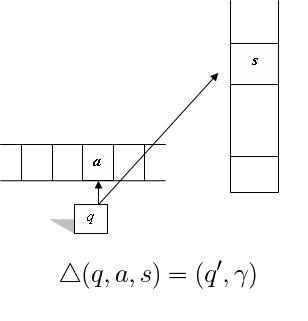
\includegraphics[width=9cm, height=6cm]{img/automata-pila.png}
		\caption{Representación de un autómata de Pila.}
		\label{fig:diagrama-pila}
		\end{center}
	\end{figure}
	\begin{figure}[H]
		\begin{center}
			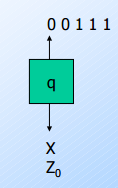
\includegraphics[width=6cm, height=6cm]{img/animacion-pila.png}
			\caption{Representación de un autómata de Pila.}
			\label{fig:pila-animacion}
		\end{center}
	\end{figure}
	\subsection{Código}
	El código fue realizado en Python 3.5.
	\\Archivo: main\_pila.py
	\begin{lstlisting}[language=Python]
	#main_pila.py
	# -*- coding: utf-8 -*-
	from __future__ import print_function
	from pila import automata
	import random

	separador = '='*50
	def iniciar():
	    continuar = True
	    while continuar:
	        opcion = imprimir_menu()
	        if opcion == 1:
	            entrada_consola()
	        elif opcion == 2:
	            ejecutar_random()
	        else:
	            break # Sal del programa
	        print('=' * 100)
	        opcion = input("Reintentar [s/n]: ")
	        if opcion.lower() != 's':
	            continuar = False

	    print('Saliendo del programa...')

	def imprimir_menu():
	    print('\n\n%sMenu%s' % (separador, separador))
	    print("""
	        1.- Entrada en consola (Manual)
	        2.- Aleatorio (Automatico)
	        3.- Salir
	    """)
	    try:
	        opcion = int(input("Selecciona una opcion valida: "))
	        return opcion
	    except Exception as e:
	        print('Error ', e)
	        return 0

	def entrada_consola():
	    texto = input("Escribe el numero binario: ")
	    animacion = ver_animacion()
	    automata(texto, animacion)

	def ver_animacion():
	    opcion = input("Ver animacion [s/n]: ")
	    if opcion == 's':
	        return True
	    else:
	        return False

	def ejecutar_random():
	    i = 0
	    longitud_random = random.randint(1, 10)
	    numero_binario = ''
	    while i < longitud_random:
	        numero_binario += random.choice(['0', '1'])
	        i += 1

	    print("El numero aleatorio es: ", numero_binario)
	    animacion = ver_animacion()
	    automata(numero_binario, animacion)

	iniciar()
	\end{lstlisting}
	Archivo: automata\_pila.py
	\begin{lstlisting}[language=Python]
	#automata_pila.py
	# -*- coding: utf-8 -*-
	from __future__ import print_function
	import time

	class Pila(object):
	    def __init__(self):
	        self.altura = -1
	        self.elementos = []

	    def vacio(self):
	        if self.altura == -1:
	            return True
	        else:
	            return False

	    def sacar(self):
	        if self.vacio():
	            return 'e'
	        else:
	            valor = self.elementos[self.altura]
	            self.altura -= 1
	            return valor

	    def meter(self, elemento):
	        self.altura += 1
	        self.elementos[self.altura:] = [elemento]

	    def mostrar(self):
	        i = self.altura
	        cadena = ''
	        while(i>-1):
	            cadena += self.elementos[i]
	            i -= 1
	        return cadena

	def automata(cadena, ver_animacion):
	    pila = Pila()
	    archivo = open('historia-pila.txt', 'w')
	    pila.meter('Zo')
	    estado = 'q'
	    cadena_aux = cadena
	    cadena = cadena + ' '
	    archivo.write('La cadena es: ' + cadena_aux + '\n')
	    for simbolo in cadena:
	        if cadena_aux == '':
	            cadena_aux = 'e'
	        if ver_animacion:
	            time.sleep(1)
	            pintar(estado, cadena_aux, pila)
	        else:
	            print('(%s, %s, %s)' %(estado, cadena_aux, pila.mostrar()), end=' |- ')
	        archivo.write('(%s, %s, %s) |- ' %(estado, cadena_aux, pila.mostrar()))
	        if estado == 'q':
	            if simbolo == '0':
	                pila.meter('X')
	            elif simbolo == '1':
	                if pila.sacar() == 'Zo':
	                    pila.meter('Zo')
	                    break
	                estado = 'p'
	            else:
	                estado = 'f'
	                break
	        elif estado == 'p':
	            if simbolo == '1':
	                if pila.sacar() == 'Zo':
	                    estado = 'f'
	                    pila.meter('Zo')
	                    break
	            elif simbolo == '0':
	                pila.meter('X')
	                cadena_aux = cadena_aux[1:]
	                break
	            elif simbolo == ' ':
	                estado = 'f'
	                if pila.mostrar() == 'Zo':
	                    break
	        cadena_aux = cadena_aux[1:]

	    if cadena_aux == '':
	        cadena_aux = 'e'
	    if ver_animacion:
	        time.sleep(1)
	        pintar(estado, cadena_aux, pila)
	    else:
	        print('(%s, %s, %s)' %(estado, cadena_aux, pila.mostrar()))
	        print('\n')
	    archivo.write('(%s, %s, %s)' %(estado, cadena_aux, pila.mostrar()))
	    if (pila.mostrar() == 'Zo') and cadena_aux == 'e':
	        print('\nCadena valida')
	        archivo.write('\nCadena valida')
	    else:
	        print('\nCadena invalida')
	        archivo.write('\nCadena invalida')
	    archivo.close()

	def pintar(estado, cadena_aux, stack):
	    pila = 'Zo'
	    if stack.mostrar() != '':
	        pila = stack.mostrar()

	    print('\n')
	    print('\n')
	    print('\n')
	    print('\n')
	    print('\n')
	    print('     %s' %cadena_aux)
	    print('     ^')
	    print('     |')
	    print('     |')
	    print('     |')
	    print('-----------')
	    print('|         |')
	    print('|    %s    |' %estado)
	    print('|         |')
	    print('-----------')
	    print('     |')
	    print('     |')
	    print('     |')
	    print('     v')
	    print('     %s' %pila)
	    print('\n')
	    print('\n')
	    print('\n')
	    print('\n')
	    print('\n')
	\end{lstlisting}
	\subsection{Pruebas}
	Pruebas de las opciones del menú.
	\\
	{\large Modo de manual.}
	\begin{figure}[H]
		\begin{center}
			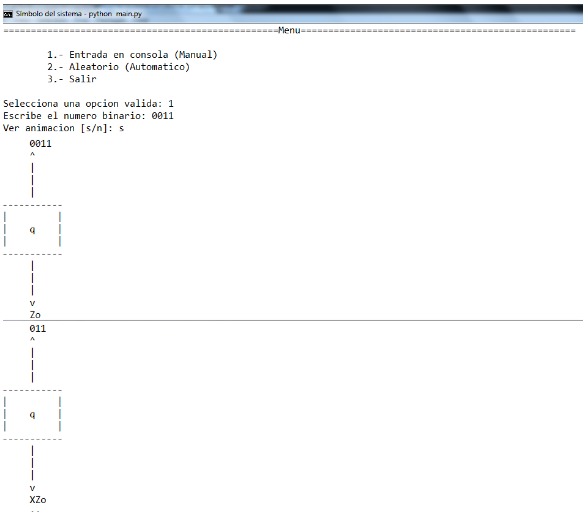
\includegraphics[width=14cm, height=12cm]{img/pila-manual-consola1.png}
			\caption{Historia del Autómata de Pila en animación 1}
			\label{fig:pila1a}
		\end{center}
	\end{figure}
	\begin{figure}[H]
		\begin{center}
			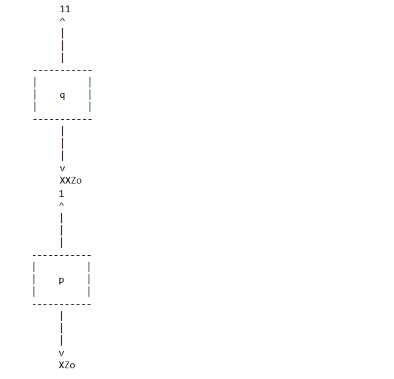
\includegraphics[width=14cm, height=10cm]{img/pila-manual-consola2.png}
			\caption{Historia del Autómata de Pila en animación 2}
			\label{fig:pila1b}
		\end{center}
	\end{figure}
	\begin{figure}[H]
		\begin{center}
			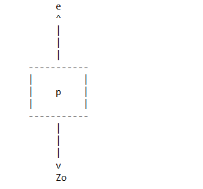
\includegraphics[width=7cm, height=7cm]{img/pila-manual-consola3.png}
			\caption{Historia del Autómata de Pila en animación 3}
			\label{fig:pila1c}
		\end{center}
	\end{figure}
	\begin{figure}[H]
		\begin{center}
			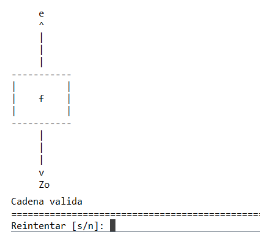
\includegraphics[width=9cm, height=8cm]{img/pila-manual-consola4.png}
			\caption{Historia del Autómata de Pila en animación 4}
			\label{fig:pila1d}
		\end{center}
	\end{figure}
	\begin{figure}[H]
		\begin{center}
			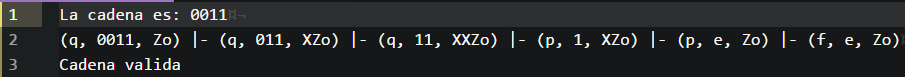
\includegraphics[width=\linewidth, height=3cm]{img/pila-manual-archivo.png}
			\caption{Historia del Autómata de Pila.}
			\label{fig:pila2}
		\end{center}
	\end{figure}
	\newpage
	{\large Modo automático}
	\begin{figure}[H]
		\begin{center}
			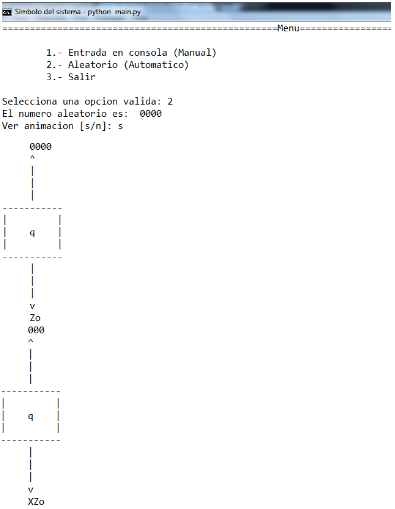
\includegraphics[width=14cm, height=16cm]{img/pila-automatico-consola1.png}
			\caption{Historia del Autómata de Pila en animación 1}
			\label{fig:pila2a}
		\end{center}
	\end{figure}
	\begin{figure}[H]
		\begin{center}
			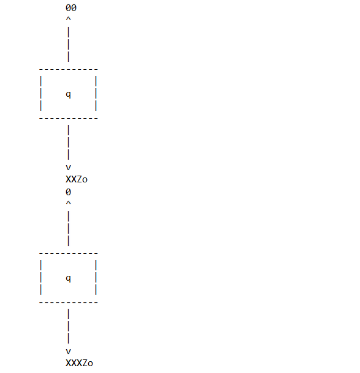
\includegraphics[width=14cm, height=12cm]{img/pila-automatico-consola2.png}
			\caption{Historia del Autómata de Pila en animación 2}
			\label{fig:pila2b}
		\end{center}
	\end{figure}
	\begin{figure}[H]
		\begin{center}
			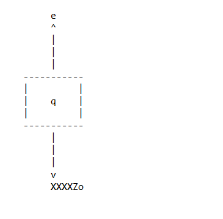
\includegraphics[width=7cm, height=7cm]{img/pila-automatico-consola3.png}
			\caption{Historia del Autómata de Pila en animación 3}
			\label{fig:pila2c}
		\end{center}
	\end{figure}
	\begin{figure}[H]
		\begin{center}
			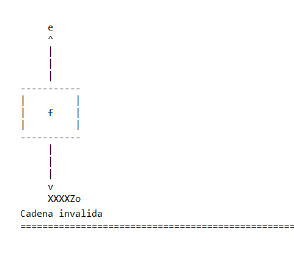
\includegraphics[width=9cm, height=8cm]{img/pila-automatico-consola4.png}
			\caption{Historia del Autómata de Pila en animación 4}
			\label{fig:pila2d}
		\end{center}
	\end{figure}
	\begin{figure}[H]
		\begin{center}
			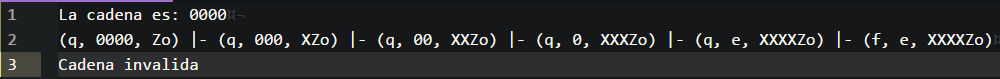
\includegraphics[width=\linewidth, height=3cm]{img/pila-automatico-archivo.png}
			\caption{Historia del Autómata de Pila en archivo.}
			\label{fig:pila4}
		\end{center}
	
	\end{figure}
